\documentclass{beamer}

\usepackage[utf8]{inputenc}
\usepackage{graphicx}
\usepackage{geometry}
\usepackage{tikz}


\usetheme[numbering=counter, progressbar=frametitle, block=fill]{metropolis}
\graphicspath{ {res/} }

\title{Linux: Grundkurs}
\subtitle{Eine Einführung in den KDE-Desktop}
\author{Paul Seidel}
\date{\today} %may change
\institute{ZKK - Universität Passau}

\begin{document}

    \maketitle

    %! Author = paulsen
%! Date = 10.09.23

\begin{frame}{Einführung}
    \section{Einführung}\label{sec:einfuhrung}

    Zu Mir:

    \begin{itemize}
        \item Studiere Internet Computing
        \item Nutze Linux seit 3 Jahren in der Uni \& Privat
        \item Benutze auch noch Windows :)
    \end{itemize}

\end{frame}

\begin{frame}{Erwartungen}
    \subsection{Erwartungen}\label{subsec:erwartungen}

    \begin{itemize}
        \item \begin{quote}
                  Linux ist was für Nerds!
        \end{quote}
        \item \begin{quote}
                  Da macht man alles in der "Hacker"-Konsole!
        \end{quote}
        \item \begin{quote}
                  Des ist mir zu viel Neuland!
        \end{quote}
    \end{itemize}

\end{frame}

\begin{frame}{Ziele}
    \subsection{Ziele}\label{subsec:ziele}


\end{frame}

\begin{frame}{Kursablauf}
    \subsection{Ablauf}\label{subsec:ablauf}

\end{frame}
    %! Author = paulsen
%! Date = 12.09.23

\begin{frame}
    \frametitle{Test}


    \section{Testsection}\label{sec:testsection}

    \begin{quote}
        Lorem ipsum dolor sit amet, consectetur adipisicing elit
    \end{quote}

    \begin{tikzpicture}
        [remember picture,overlay,shift={(current page.north east)}]
        \node[anchor=north east,xshift=-7cm,yshift=-2.5cm]{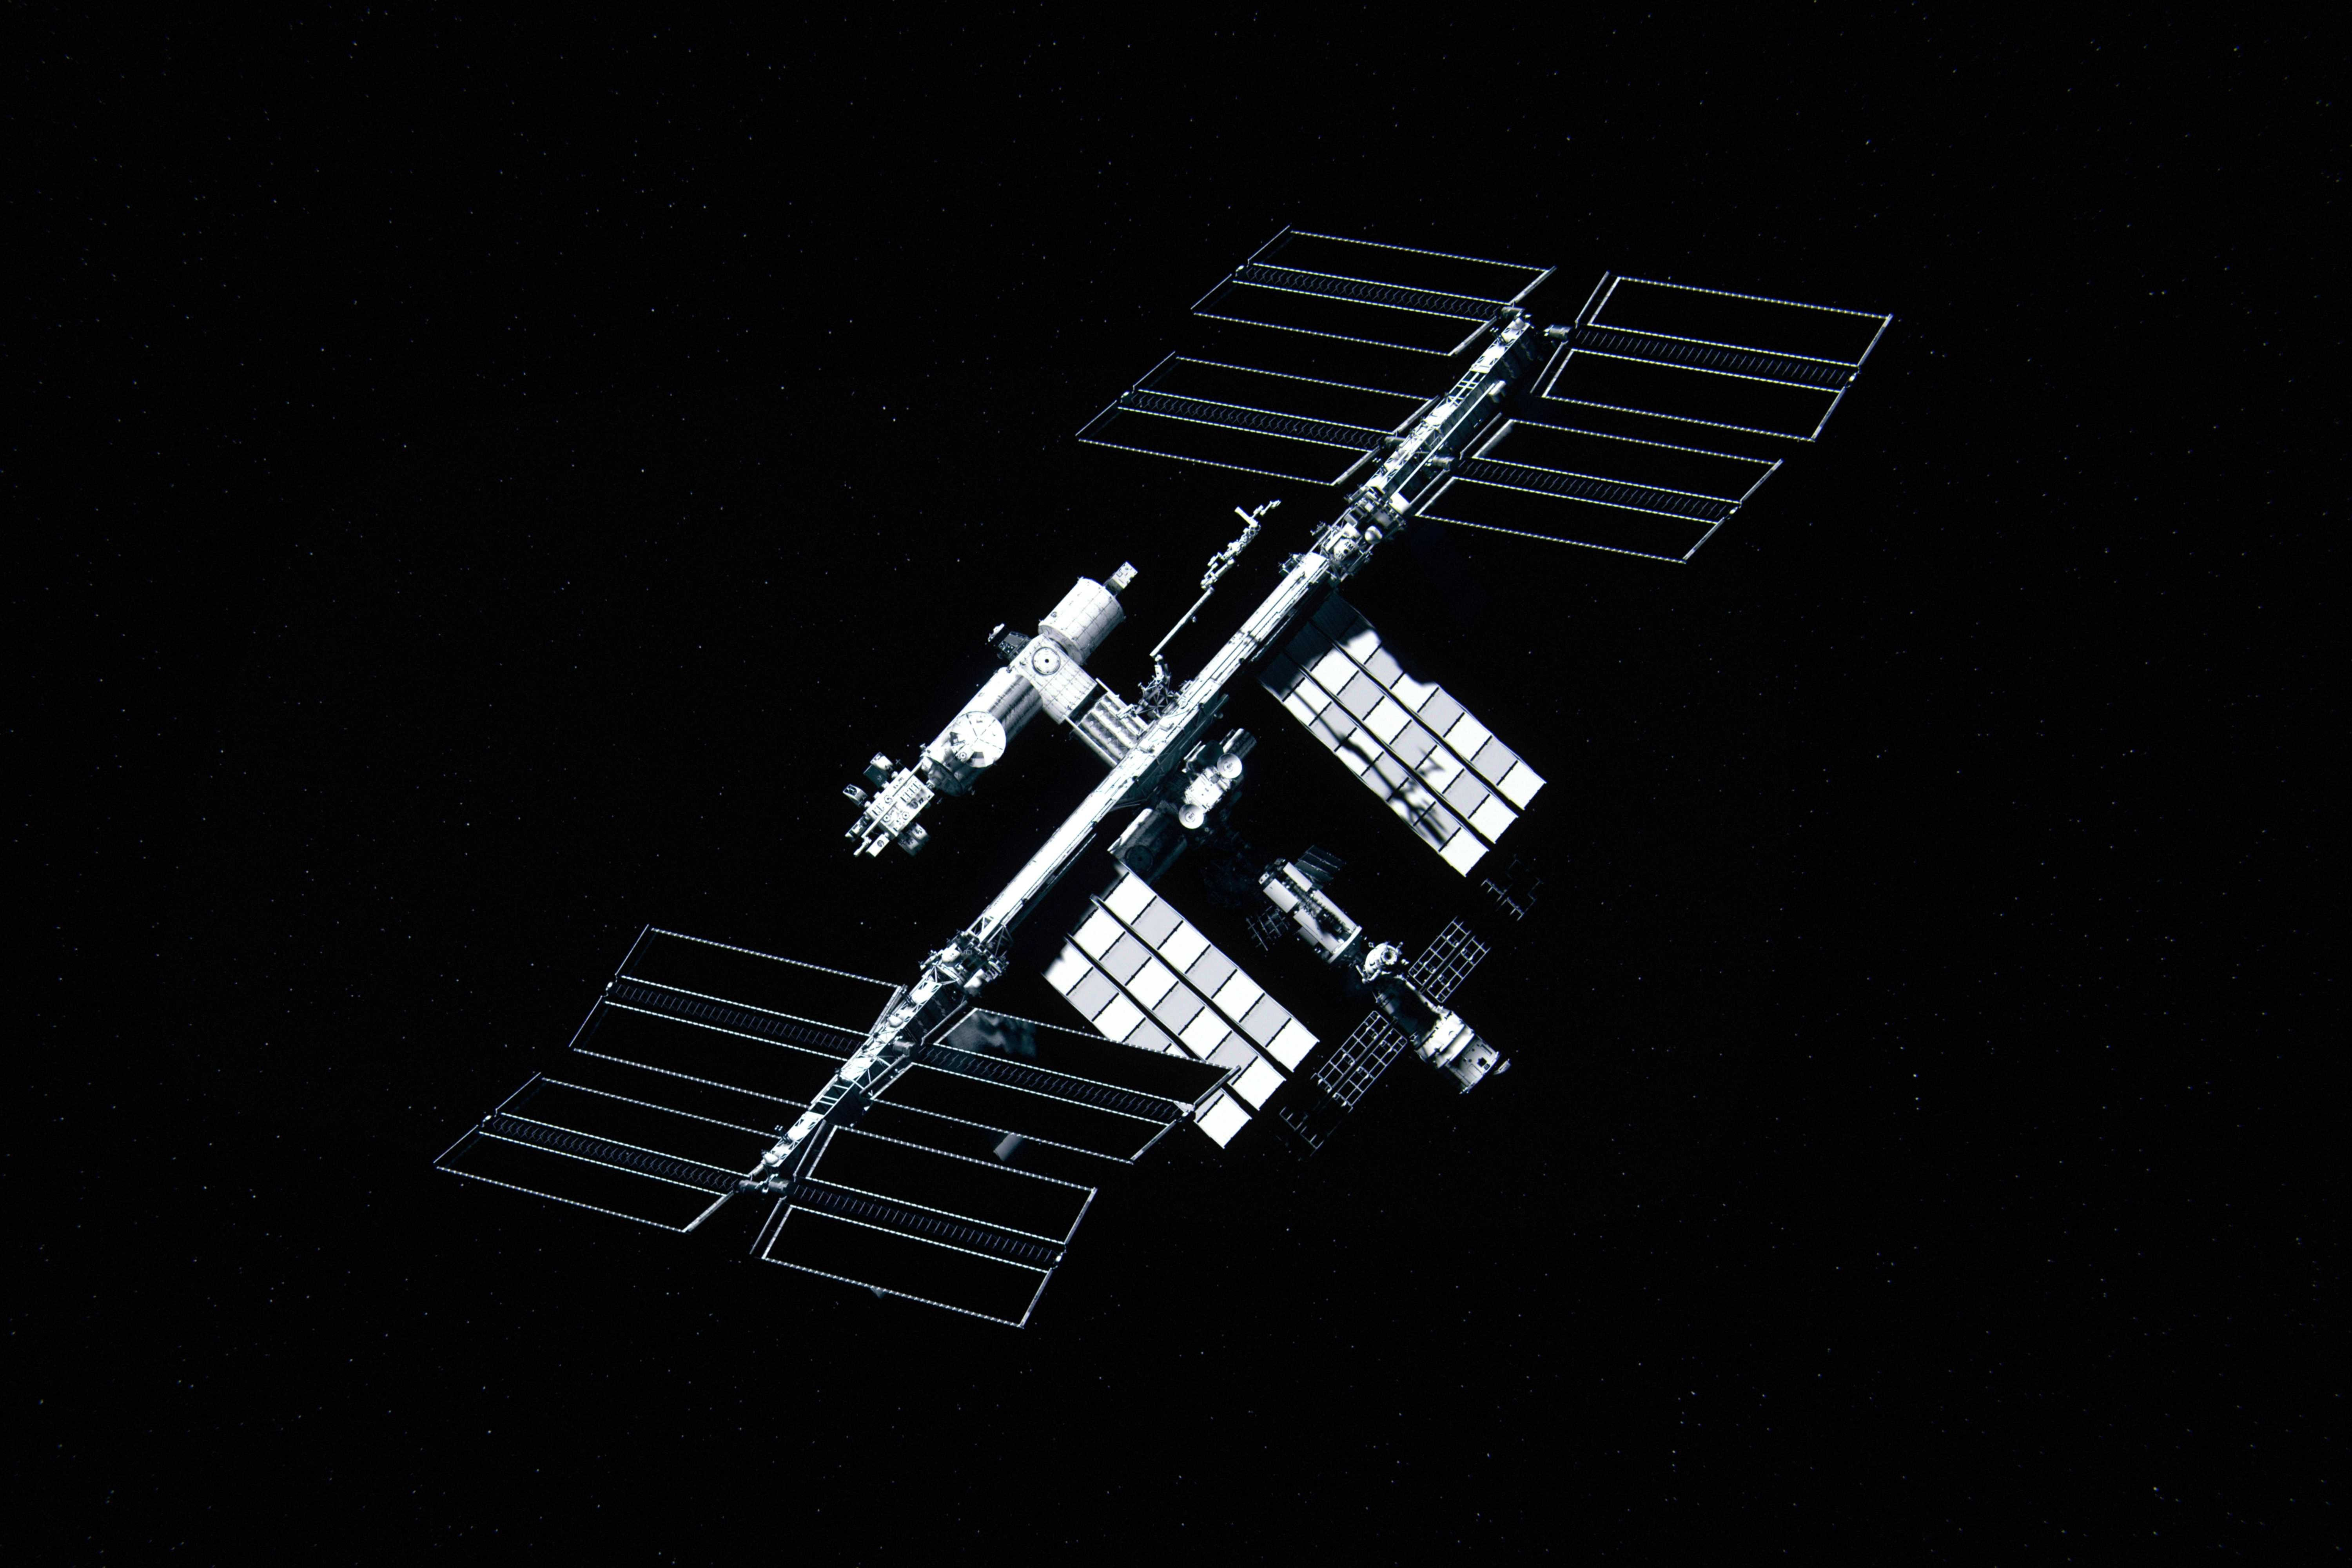
\includegraphics[width=2cm]{ISS}};
        \node[anchor=north east,xshift=-5cm,yshift=-2.5cm]{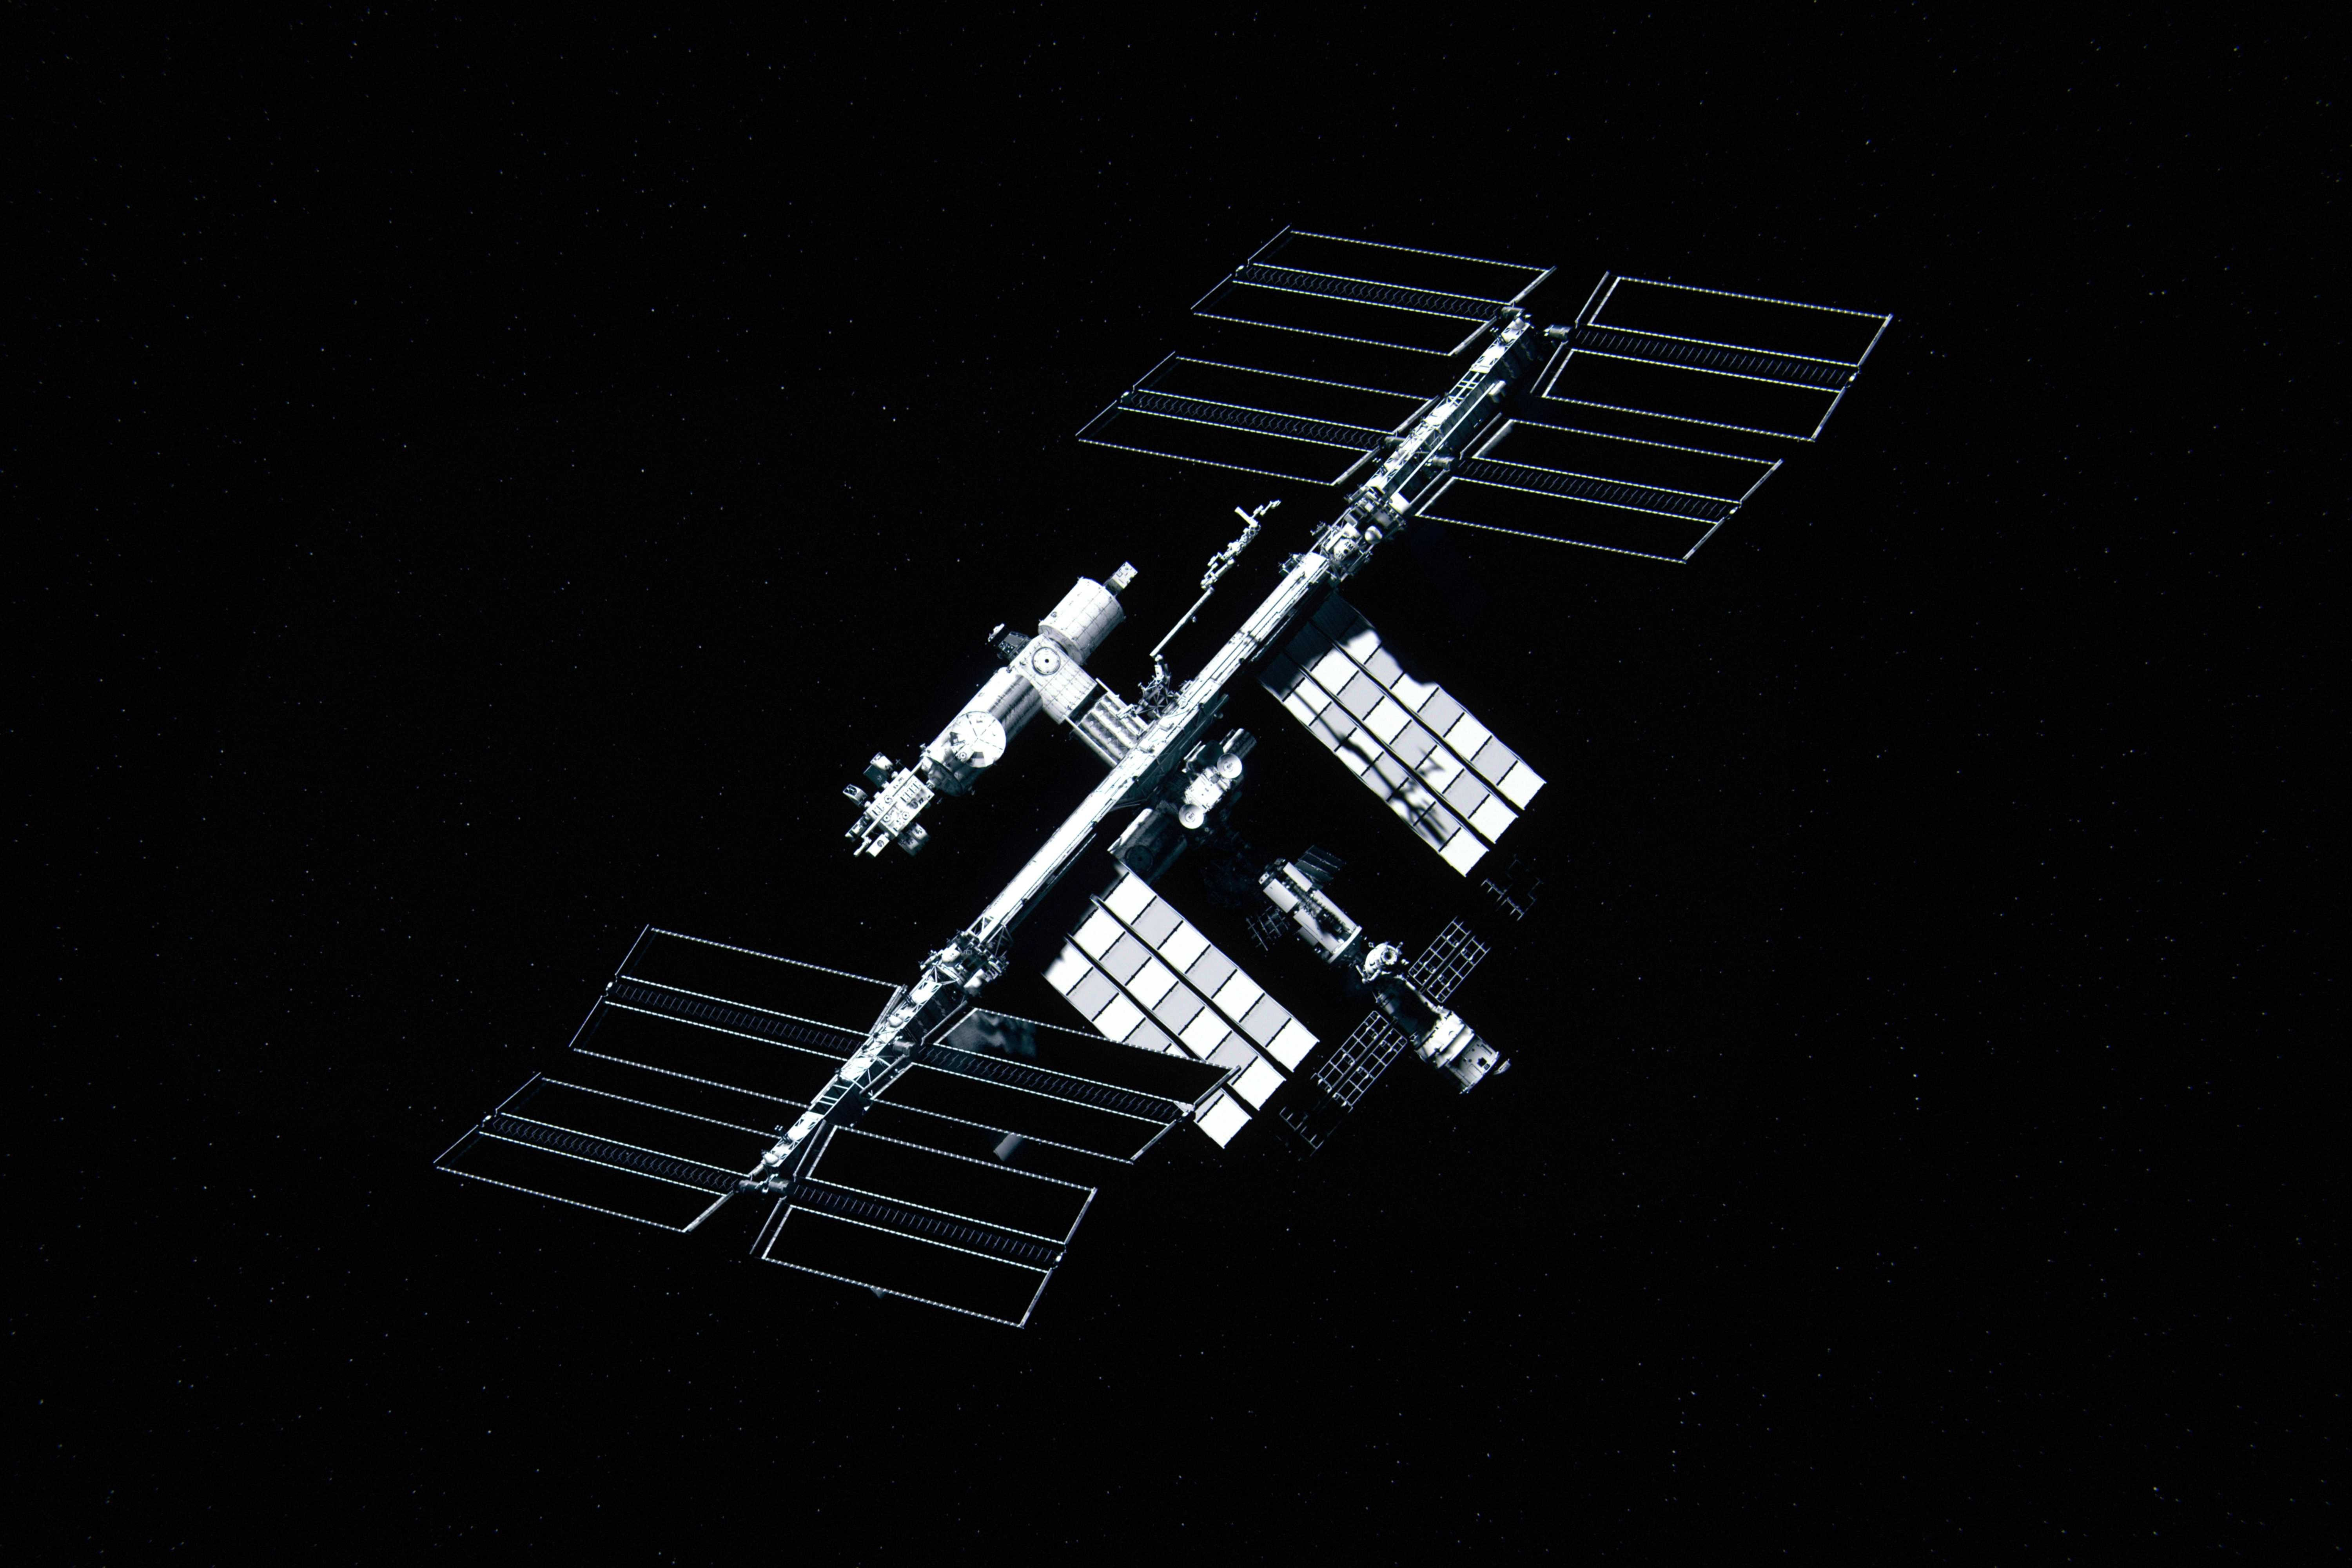
\includegraphics[width=3cm]{ISS}};
        \node[anchor=north east,xshift=-1cm,yshift=-2.5cm]{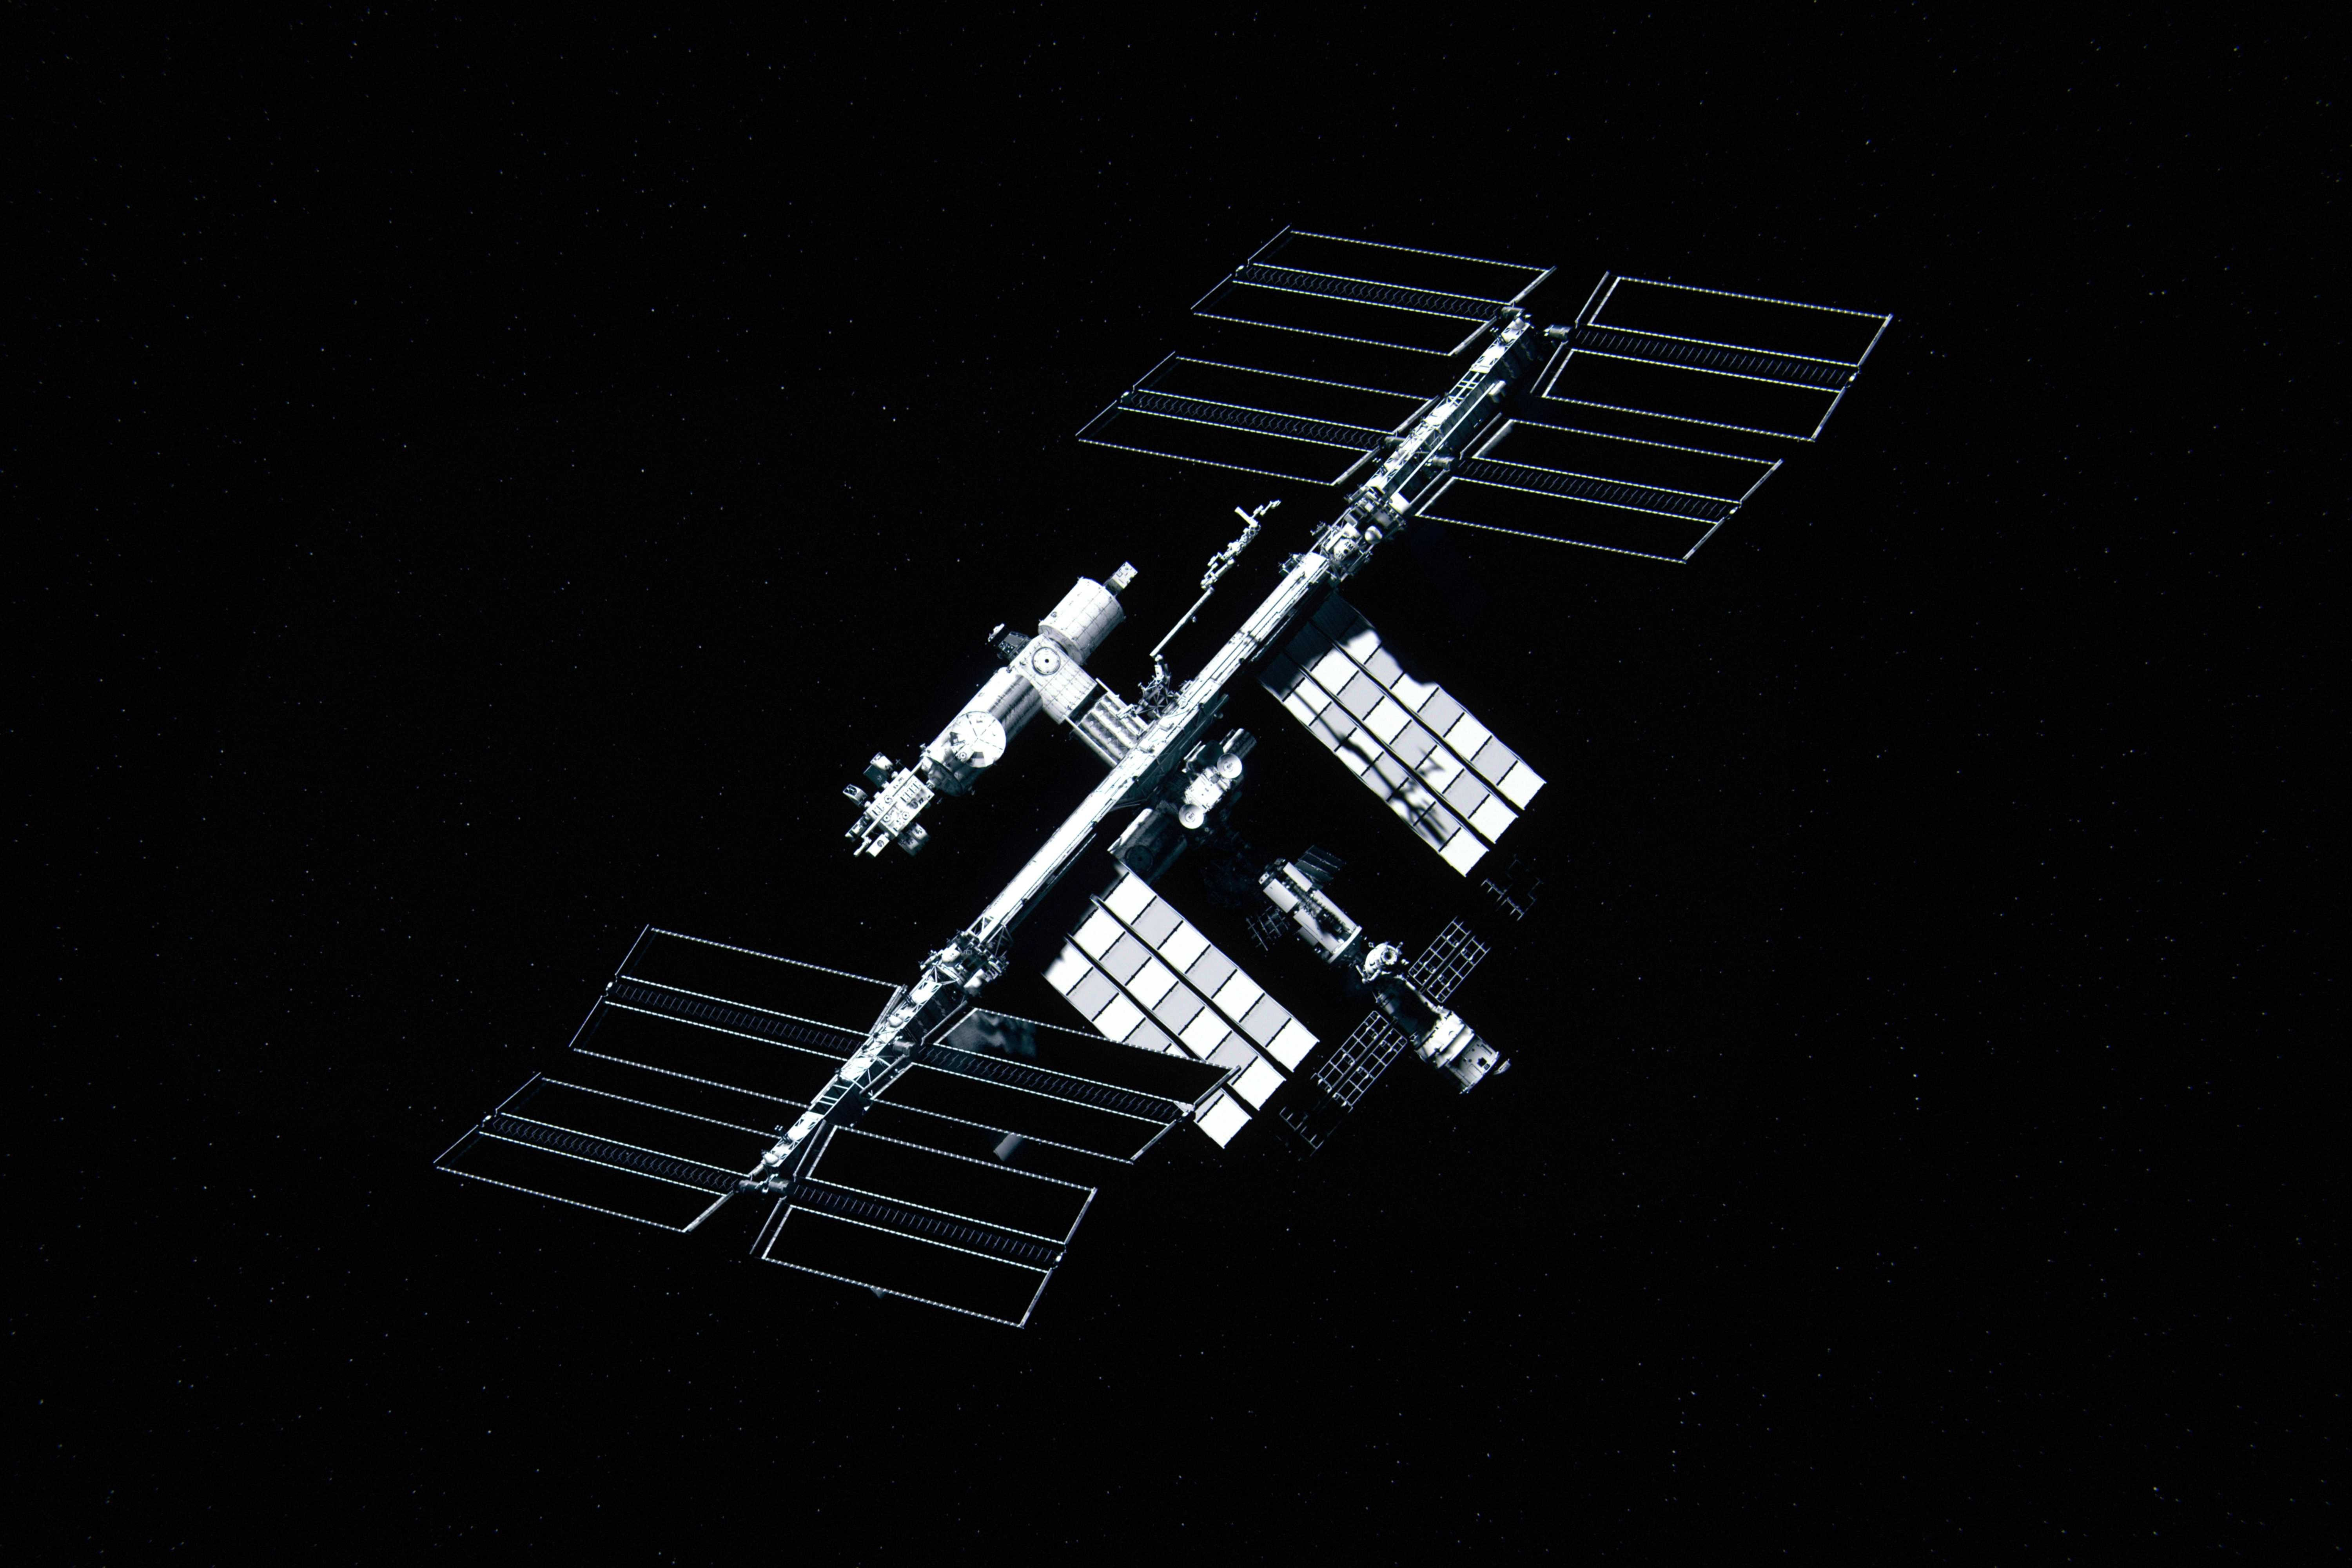
\includegraphics[width=5cm]{ISS}};
    \end{tikzpicture}

    \subsection{Listen}\label{subsec:Listen}
    \begin{itemize}
        \item[!.] Eintrag
        \begin{enumerate}
            \item Test123
        \end{enumerate}
        \item Descriptions
        \begin{description}
            \item[Thema] Schilderung
        \end{description}
    \end{itemize}

    \subsection{Blöcke}\label{subsec:Blocke}
    \begin{exampleblock}{Beispiel 1}
        Die ISS ist schön
    \end{exampleblock}
    \begin{alertblock}{Fun Fact}
        Die ISS läuft mit Linux.
    \end{alertblock}

\end{frame}

    \begin{frame}[standout]
        Danke
    \end{frame}

\end{document}